\chapter[Código]{Código}
\label{Chap5}

\section{Creación de Spiders}
Una vez instalado Scrapy, en nuestro directorio escogido escribimos el siguiente comando para generar un nuevo proyecto de Scrapy.

\begin{verbatim}
	scrapy startproject miproyecto
\end{verbatim}

Nos creara un nuevo directorio con el siguiente contenido.

\begin{figure} [h!]
	\centering
	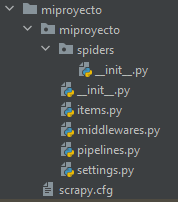
\includegraphics[width=0.3\textwidth]{fig/estructura_proyecto_scrapy.png}
	\caption[Estructura del proyecto recién creado]{Estructura del proyecto recién creado}
	\label{fig:ej11}
\end{figure}

Primero entraremos en el directorio recientemente creado y luego ejecuteremos el comando encargado de crear la Spider.

\begin{verbatim}
	cd miproyecto
	scrapy genspider mispider webausar.com
\end{verbatim}

En caso de no especificar el protocolo usado por la web Scrapy asumirá que usa HTTPS.
\newline
Tras ejecutar el comando la Spider habrá sido generada dentro de la carpeta spiders.

\begin{figure} [h!]
	\centering
	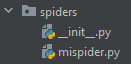
\includegraphics[width=0.3\textwidth]{fig/primera_spider.png}
	\caption[Directorio de almacenamiento de las Spider]{Directorio de almacenamiento de las Spider}
	\label{fig:ej12}
\end{figure}

Una vez abierto el archivo vemos que dispone del siguiente código.

\begin{lstlisting}[language=Python]
	import scrapy
	
	
	class MispiderSpider(scrapy.Spider):
		name = "mispider"
		allowed_domains = ["webausar.com"]
		start_urls = ["https://webausar.com"]
	
	def parse(self, response):
		pass
\end{lstlisting}

Como podemos ver Scrapy usa una programación orientada a objetos, siendo cada Spider una clase representada dentro del proyecto.\newline
Analizando las variables definidas vemos las siguientes, name, nombre por el que debemos referenciar la Spider a la hora de ejecutarla; allowed\_domains, indica que dominios podemos visitar, negando la entrada a cualquier dominio que no este definido en ella, es importante no especificar protocolo, de esta manera funcionara para cualquier web ya sea HTTP como HTTPS que pertenezca a ese dominio, de lo contrario se limitara al protocolo indicado; start\_urls, URL inicial sobre la que se hará la request de petición de datos.\newline
El método parse es aquel al que se envía la respuesta obtenida de la web, para realizar el filtrado de la información, quedándote unicamente con la deseada. Este método es invocado automáticamente por la Spider, sin necesidad real de hacerlo tu manualmente.

\subsection{Proceso de obtención de datos}
Para poder realizar es la extracción de los datos, primero debemos ir a la web deseada e inspeccionar su estructuración. Para ello como ejemplo vamos a usar la web de aemet.\newline

\begin{figure} [H]
	\centering
	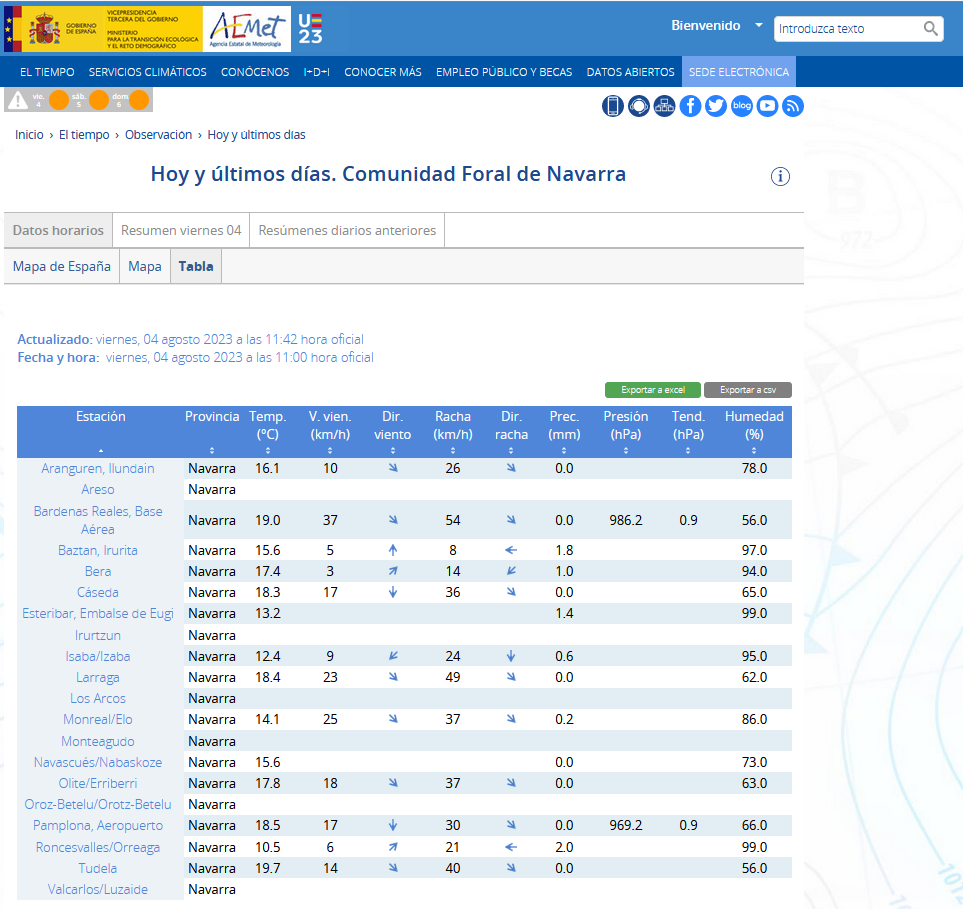
\includegraphics[width=0.8\textwidth]{fig/code_aemet.png}
	\caption[URL de inicio para obtener los códigos de las estaciones de Aemet]{Web de Aemet para obtención de datos}
	\label{fig:ej13}
\end{figure}

Una vez encontrada la web deseada, accediendo mediante el F12 a la herramienta de inspección, buscamos el elemento representativo del dato deseado. En nuestro caso queremos obtener tanto el nombre como el código de la estación. Ambos se encuentran en el mismo elemento que forma la primera columna de la tabla.\newline

\begin{figure} [H]
	\centering
	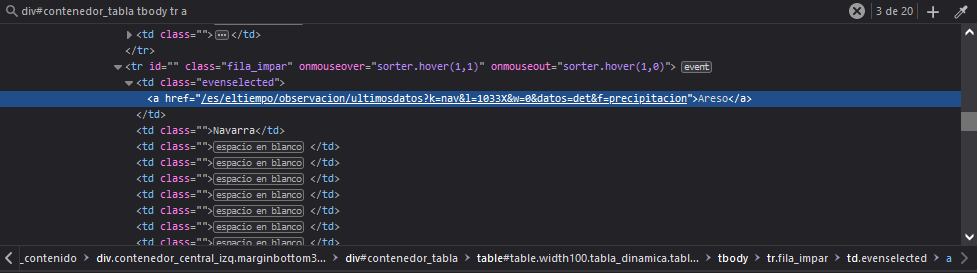
\includegraphics[width=0.9\textwidth]{fig/inspector.png}
	\caption[Inspector de webs de Chrome]{Inspector de webs}
	\label{fig:ej14}
\end{figure}

Como en este caso es posible filtrar fácilmente los datos, los obtendremos todos directamente, aunque lo más común sería obtener las filas primero para luego iterar por cada una de ellas. Para obtenerlos podemos hacerlo mediante el selector de XPath como con el de CSS.\newline

\begin{verbatim}
	rows = response.xpath('//div[@id="contenedor_tabla"]/table/tbody/tr/td/a')
	ó
	rows = response.css("div#contenedor_tabla tbody tr a")
\end{verbatim}

Esto nos devuelve una lista de objetos tipo Selector, cosa que nos permite conforme vamos iterando por cada elemento volver a usar un selector para filtrar unicamente los datos deseados. En nuestro caso.

\begin{verbatim}
	path = rows[i].xpath("@href").get()
	name = rows[i].xpath("./text()").get()
	ó
	path = rows[i].css("*::attr(href)").get()
	name = rows[i].css("*::text").get()
\end{verbatim}

De esta forma, mediante el uso de la función get(), pasamos de tener un objeto Selector a un String. El uso de get() sobre una lista devuelve el primer elemento, en caso de querer transformar toda la lista el método a usar es getall().\newline
\newline
Finalmente, como de la URL obtenida,
\begin{verbatim}
	'/es/eltiempo/observacion/ultimosdatos?k=nav&l=9263X&w=0&datos=det&f=precipitacion'
\end{verbatim}
solo nos interesa el código de la estación (parámetro l de la query), lo filtraremos.
\begin{verbatim}
	code = path.split('&')[1].split('=')[1]
\end{verbatim}

\subsection{Guardado de datos}
Scrapy almacena todos los datos en forma de múltiples diccionarios, tantos como webs usadas. Para acceder a esta información Scrapy nos proporciona dos alternativas, el uso de Items junto a ItemLoaders, siendo clases especificas de Scrapy o, mediante la palabra reservada yield de Python, siendo esta la opción elegida debido a su fácil implementación.
De esta forma escribiremos.
\begin{verbatim}
	yield {
		'estacion': name,
		'codigo': path.split('&')[1].split('=')[1],
	}
\end{verbatim}
Actualmente si se ejecuta la Spider nos imprimiría los datos obtenidos por pantalla, aunque pueden ser almacenados en un fichero tanto CSV como JSON, a la hora de ejecutar la Spider añadiendo en el comando "-o nombre.csv ó -o nombre.json".\newline
Para un uso ligero de forma manual esa alternativa es más que suficiente, pero en nuestro caso, al querer ejecutarlas de forma automática mediante el uso de Runners, debemos implementar una variable llamada custom\_settings para cada una de las Spider. Esta permite, sin la necesidad de modificar el archivo settings.py, añadir configuraciones o dependencias independientes en las Spiders.
\begin{lstlisting}[language=Python]
	custom_settings = {
		'FEEDS': {
			'JSONs/RawCode/codigos_aemet.json': {
				'format': 'json',
				'encoding': 'utf-8',
				'overwrite': True,
			}
		}
	}
\end{lstlisting}
Con esto indicamos que, en la ruta especificada, nos almacene un fichero JSON utf-8 y, que cada vez que se llame a esta Spider sobre-escriba el fichero anterior.

\subsection{Spider básica}
Una vez obtenemos los datos y los podemos almacenar, ya estaria nuestra Spider básica terminada.
\begin{lstlisting}
	import scrapy
	
	
	class AemetCodeSpider(scrapy.Spider):
		name = "aemet_code"
		allowed_domains = ["www.aemet.es"]
		start_urls = ["https://www.aemet.es/es/eltiempo/observacion/"
		"ultimosdatos?k=nav&w=0&datos=det&x=h24&f=precipitacion"]
		custom_settings = {
			'FEEDS': {
				'JSONs/RawCode/codigos_aemet.json': {
					'format': 'json',
					'encoding': 'utf-8',
					'overwrite': True,
				}
			}
		}
	
	def parse(self, response):
		rows = response.css("div#contenedor_tabla tbody tr a")
		
		for row in rows:
		path = row.xpath("@href").get()
		name = row.xpath("./text()").get()
		code = path.split('&')[1].split('=')[1]
		
		yield {
			'estacion': name,
			'codigo': code,
		}
\end{lstlisting}
